\section{Experiments}
\label{sec:experiments}
We answer the following questions in our experiments:
1. Sampling, Scaling, and Speeding.
2. Approximation Guarantees.
3. Budget vs. Infected.
4. Characterizing structure of the solution.

\subsection{Dataset and Methods}
We experiment with four very different kinds of networks, three random and one real, in order to fully explore the effect of network structure on the the results. We consider two random networks, namely the small world 
\cite{Kleinberg00thesmall-world}, and preferential attachment \cite{Barabasi509} models. Finally, we consider a synthetic agent based population for Montgomery County, VA, constructed by a first principles approach by \cite{barrett:wsc09,eubank:nature04}. This has been used in several public health studies, e.g., \cite{singh:bmc19}. This network has a rich set of demographic attributes for each node, e.g., age, gender, and income.

\noindent
\textbf{Methods.}
We use \algo{} with one time step (i.e., $\mathcal{T}=\{0\}$, also referred to as single stage), or two time steps (i.e., $\mathcal{T}=\{0, T\}$, referred to as two stage, with $t=0$ being the first stage, and $t=T$ being the second stage). For the single stage problem, we use the strategy of picking nodes based on highest degree or eigenscore, which is the component in the first eigenvector of the graph's adjacency matrix as baselines \cite{tong:cikm12}.
There are no prior baselines for temporal vaccination. 

\begin{table}[!h]
\centering
\begin{tabular}{llll}
\hline
 \textbf{Dataset} & \textbf{Nodes} & \textbf{Edges}   \\ \hline
 Montgomery & 70729 & 198138 \\
Preferential2 (PA2) & 100000 & 199996 \\
 Small World (SW) & 2500 & 14833 \\   
 Preferential1 (PA1) & 1000 & 1996 \\ \hline
\end{tabular}
\caption{Description of datasets}
\label{tab:datasets}
\end{table}

\subsection{Sampling, Scaling, and Speeding}
\textbf{Impact of varying $p$ on the average infections}
In this experiment, for each graph, we sample 100 subgraphs varying the probability of infection $p$. The expected number of sources are set to 10. Figure \ref{fig:PA_ar} shows, for the graph PA, that the average percentage of infections is low (within 30\% of the population) for $p \leq 0.25$, medium (within 60\%) for $0.25 < p < 0.4$, high ($\geq 60\%$) for $p \geq 0.4$. Figure \ref{fig:montgo_ar} shows that with a very small probability close to $0.1$, the average percentage of infections rise above 55\% (medium) of the total population. 

\begin{figure}[!h]
    \centering
    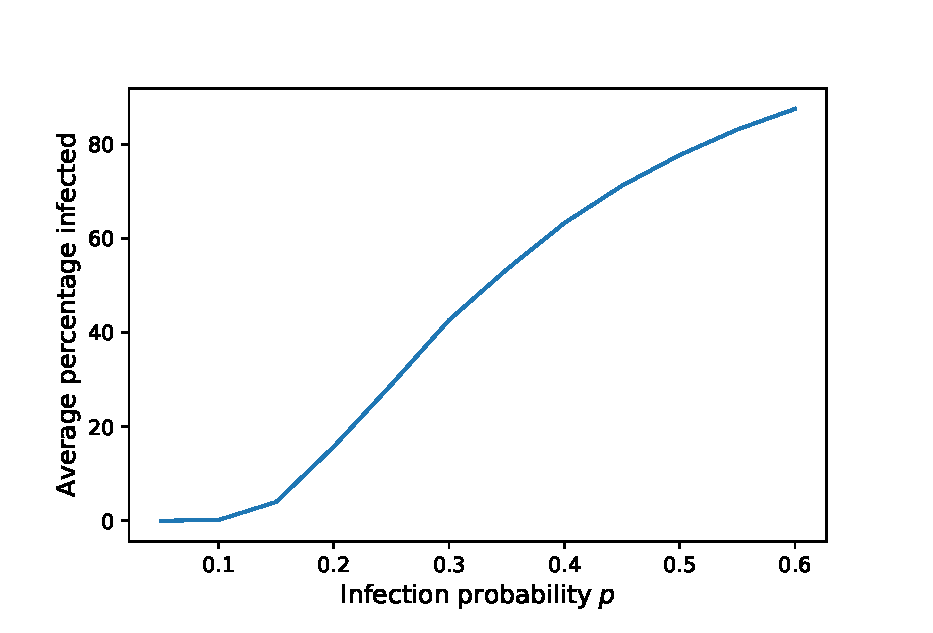
\includegraphics[scale = 0.55]{Figuresnew/PA_attackrates.eps}
    \caption{Preferential: p vs avg. percent infected.)}
    \label{fig:PA_ar}
\end{figure}

\begin{figure}[!h]
    \centering
    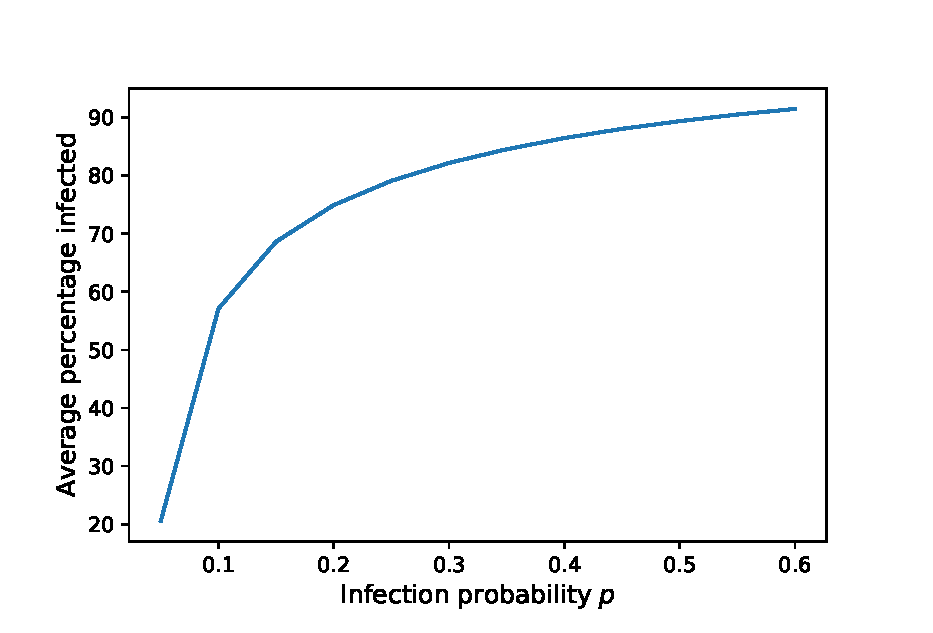
\includegraphics[scale = 0.55]{Figuresnew/montgo_attackrates.eps}
    \caption{Montgomery: p vs avg. percent infected.}
    \label{fig:montgo_ar}
\end{figure}



\begin{figure}[!h]
    \centering
    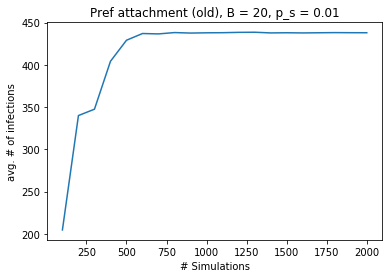
\includegraphics[scale = 0.6]{Figuresnew/simulations.png}
    \caption{Simulation vs average infected (Preferential Attachment)}
    \label{fig:pa_simvsavg}
\end{figure}
 
\begin{figure}[!h]
    \centering
    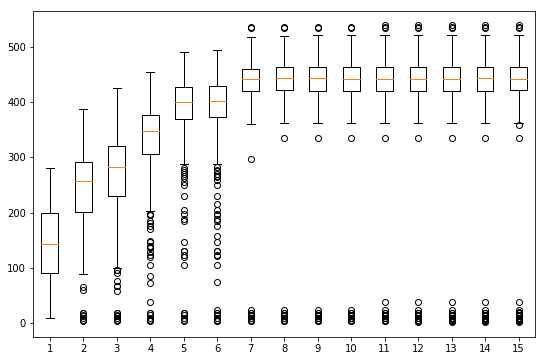
\includegraphics[scale = 0.4]{Figuresnew/boxplotpa.png}
    \caption{Box-plot: Simulation vs average infected (Preferential Attachment). X-axis: number of simulations (in 100s). Y-axis the number of infected.}
    \label{fig:pa_boxplot}
\end{figure}
\subsection{Performance Guarantees}
Will have plots for the larger datasets for both comparison with baselines and approximation guarantees.
\subsubsection{Comparison to baselines}
\subsubsection{Approx Ratio}
\begin{figure}[!h]
    \centering
    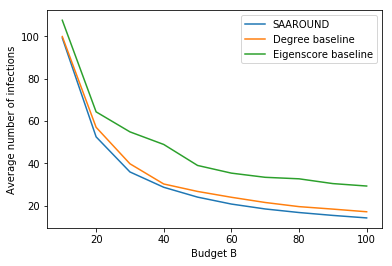
\includegraphics[scale = 0.55]{Figuresnew/pa1_approx.png}
    \caption{Preferential1: Comparison of \algo{} with the degree and eigenscore based baselines.}
    \label{fig:pa1approx}
\end{figure}

\
%\subsection{Approximation Guarantees}


%\subsection{Characterizing Structure of Solution}

